\documentclass[pdftex,12pt,xcolor=svgnames]{beamer}

\mode<presentation>
{
  \usetheme{boxes}
  \usecolortheme[named=MidnightBlue]{structure}
  %\setbeamercolor{normal text}{bg=NavajoWhite!20}
  \usefonttheme{serif}
  \setbeamertemplate{navigation symbols}{}
  % Show frame number and author name in footline
  \setbeamertemplate{footline}[frame number]
  \addtobeamertemplate{footline}{\quad\textcolor{gray}{James Robert Lloyd}}{}
  % Set frame titles in small capitals
  \setbeamerfont{frametitle}{shape=\scshape,family=\rmfamily}
  \setbeamercolor{frametitle}{bg=gray!60!white,fg=black}
  % Alerted text: blue (uncomment second line if theme sets alerted text to bold)
  \setbeamercolor{alerted text}{fg=blue}
  %\setbeamerfont*{alerted text}{}
  \setbeamertemplate{bibliography item}[text] %{\hbox{\donotcoloroutermaths$\blacktriangleright$}}
  \setbeamertemplate{bibliography entry title}{}
  \setbeamertemplate{bibliography entry author}{}
  \setbeamertemplate{bibliography entry note}{}
  \setbeamertemplate{bibliography entry location}{}

}
\usepackage[english]{babel}
\usepackage[latin1]{inputenc}
\usepackage{times}
\usepackage[T1]{fontenc}
\usepackage{hyperref}
\usepackage{multimedia}
\usepackage{eepic}
\usepackage{graphicx}
%\usepackage[nohug]{latexinclude/diagrams}
\usepackage{tikz}
\usetikzlibrary{calc}

%% \newcommand{\footlineextra}[1]{
%%     \begin{tikzpicture}[remember picture,overlay]
%%         \node[yshift=1.5ex,anchor=south east] at (current page.south east)
%% {#1};
%%     \end{tikzpicture}
%% }

\newcommand{\footlineextra}[1]{
    \begin{tikzpicture}[remember picture,overlay]
        \node[xshift=-5ex,yshift=-0.5ex,anchor=south east] at (current page.south east)
             {\mbox{\tiny \textcolor{MidnightBlue}{#1}}};
    \end{tikzpicture}
}

\def\sectionframe#1{
  {
    \setbeamertemplate{footline}{\empty}
    \begin{frame}{}
      \begin{center}
        \huge\sc #1
      \end{center}
    \end{frame}
  }
}


\usepackage{etex}

\usepackage{tabularx}
\usepackage{multirow}
\usepackage{../include/picins}
\usepackage{../include/preamble}
\usepackage{setspace}
\usepackage{xcolor}
\usepackage{tikz}

\usetikzlibrary{shapes.geometric,arrows,chains,matrix,positioning,scopes,calc,shapes.arrows}

%%%%%%%%%%%%%%%%%%%%%%%%%%%%%%%%%%%%%%%%%%%
%
% Some look and feel definitions
%
%%%%%%%%%%%%%%%%%%%%%%%%%%%%%%%%%%%%%%%%%%%

\setlength{\columnsep}{0.03\textwidth}
\setlength{\columnseprule}{0.0018\textwidth}
\setlength{\parindent}{0.0cm}
  
\tikzstyle{mybox} = [draw=white, rectangle]
\tikzset{hide on/.code={\only<#1>{\color{white}}}}

\definecolor{camlightblue}{rgb}{0.601 , 0.8, 1}
\definecolor{camdarkblue}{rgb}{0, 0.203, 0.402}
\definecolor{camred}{rgb}{1, 0.203, 0}
\definecolor{camyellow}{rgb}{1, 0.8, 0}
\definecolor{lightblue}{rgb}{0, 0, 0.80}
\definecolor{white}{rgb}{1, 1, 1}
\definecolor{whiteblue}{rgb}{0.80, 0.80, 1}

\newcolumntype{x}[1]{>{\centering\arraybackslash\hspace{0pt}}m{#1}}
\newcommand{\tabbox}[1]{#1}

\hypersetup{colorlinks=true,citecolor=blue}

%%%%%%%%%%%%%%%%%%%%%%%%%%%%%%%%%%%%%%%%%%%
%
% The talk
%
%%%%%%%%%%%%%%%%%%%%%%%%%%%%%%%%%%%%%%%%%%%

\title{The Automatic Statistician Project}

\author{
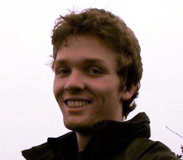
\includegraphics[height=0.16\textwidth]{../figures/JamesLloyd4}
\qquad
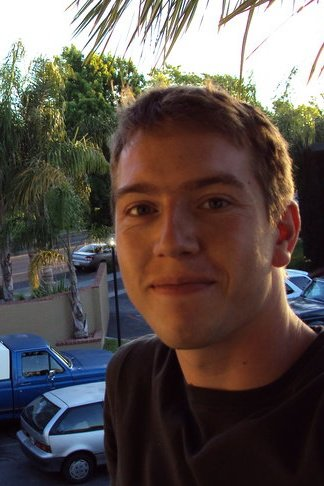
\includegraphics[height=0.16\textwidth, trim=20mm 25mm 0mm 25mm, clip]{../figures/david2}
\qquad
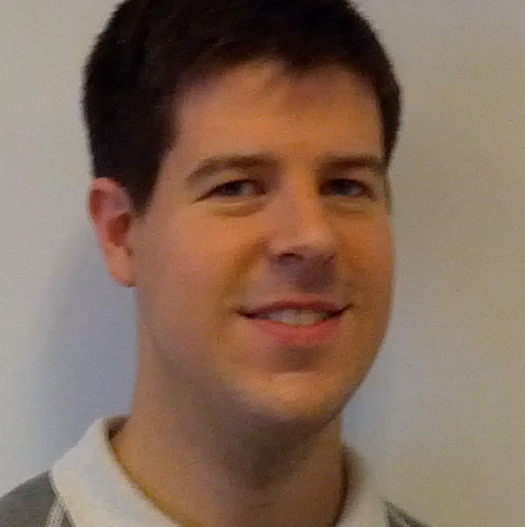
\includegraphics[height=0.16\textwidth]{../figures/roger-photo}
\\
James Robert Lloyd\textsuperscript{1}, David Duvenaud\textsuperscript{2}, Roger Grosse\textsuperscript{3},\\
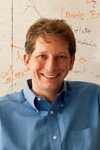
\includegraphics[height=0.16\textwidth, trim=0mm 7mm 0mm 0mm, clip]{../figures/josh2}
\qquad
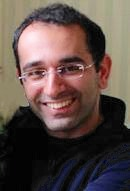
\includegraphics[height=0.16\textwidth]{../figures/zg2}\\
Joshua Tenenbaum\textsuperscript{4}, Zoubin Ghahramani\textsuperscript{1}
}

\institute{
1: University of Cambridge,
2: Harvard University\\
3: University of Toronto,
4: Massachusetts Institute of Technology
}

\begin{document}

\frame[plain] {
\titlepage
}

\begin{frame}{There is a growing need for data analysis}
  \begin{itemize}
    \item We live in an era of abundant data
    \vspace{\baselineskip}
    \item The McKinsey Global Institute claim
    \begin{itemize}
      \item \emph{``The United States alone faces a shortage of 140,000 to 190,000 people with analytical expertise and 1.5 million managers and analysts with the skills to understand and make decisions based on the analysis of big data.''}
    \end{itemize}
    \vspace{\baselineskip}
    \item Diverse fields increasingly relying on expert statisticians, machine learning researchers and data scientists \eg
    \begin{itemize}
       \item Discovery of novel interactions in gene expression data
       \item Automatically identifying different types of galaxy
       \item \ldots
     \end{itemize}
  \end{itemize}
\end{frame}

\begin{frame}{Goals of the automatic statistician project}
  \begin{itemize}
    \item Provide a set of tools for understanding data that require minimal expert input
    \begin{itemize}
      \item Aiming to speed up mechanistic parts of data analysis
      \item Not trying to replace humans any time soon!
      \item The meticulous behaviour of a machine can sometimes identify patterns that might otherwise be overlooked
    \end{itemize}
    \vspace{\baselineskip}
    \item Uncover challenging research problems in \eg
    \begin{itemize}
      \item Automated inference
      \item Model construction and comparison
      \item Data visualisation and interpretation
      \item Model checking / criticism
    \end{itemize}
  \end{itemize}
\end{frame}

\begin{frame}{We haven't done everything yet!}
  \begin{itemize}
    \item The entirety of data science / statistics / machine learning is vast
    \vspace{\baselineskip}
    \item A complete system will have to address:
    \begin{itemize}
      \item Big data
      \item Messy data
      \item Rich models
      \item Interpretability
      \item Good scientific philosophy
      \item Causality
      \item User interaction
      \item \dots
    \end{itemize}
    \vspace{\baselineskip}
    \item Short term success for the project is defined as automating any part of the pipeline that people find useful
  \end{itemize}
\end{frame}

\begin{frame}{Even simple models can be helpful}
  \begin{center}
    \begin{tikzpicture}[node distance = 0.25\textwidth]
  \begin{scope}[yshift=0\textwidth]
    \node (raw_1) at (0, 0) {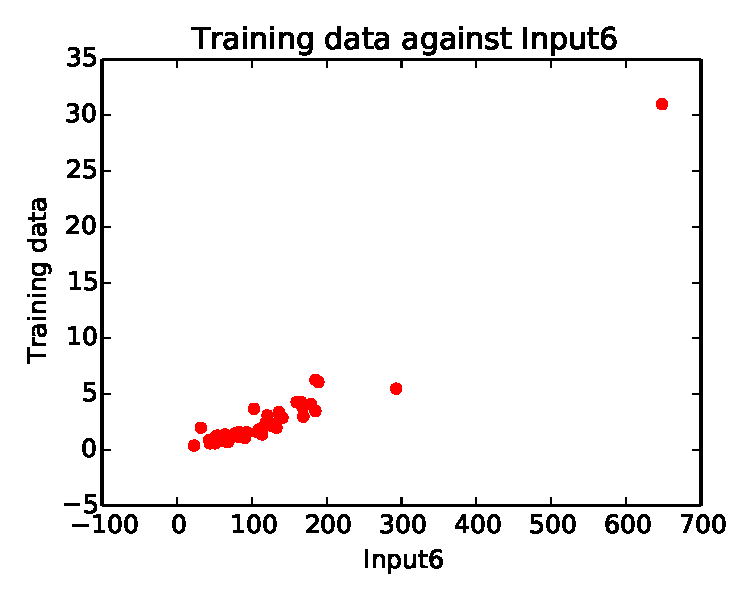
\includegraphics[width=0.25\textwidth]{../figures/auto-stat-lin-ex/lin-train-Input6.pdf}};
    \node (raw_2) [right of=raw_1] {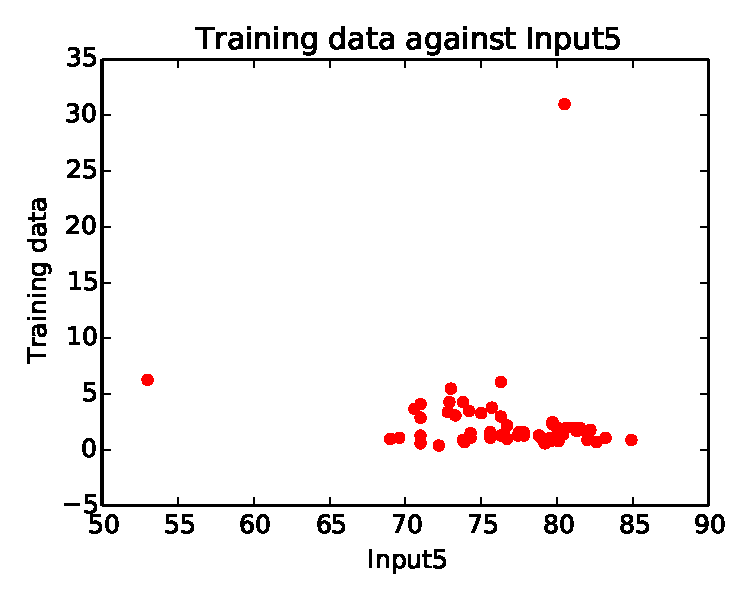
\includegraphics[width=0.25\textwidth]{../figures/auto-stat-lin-ex/lin-train-Input5.pdf}};
    \node (raw_3) [right of=raw_2] {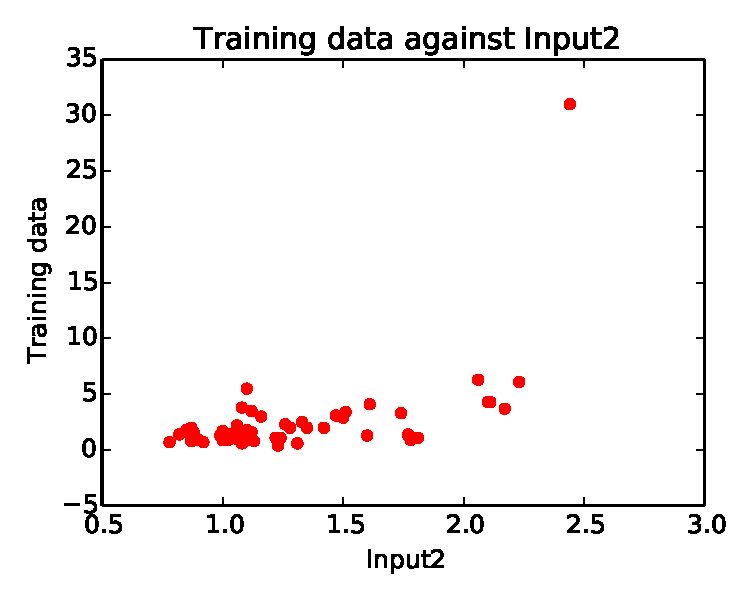
\includegraphics[width=0.25\textwidth]{../figures/auto-stat-lin-ex/lin-train-Input2.pdf}};
    \node (raw_4) [right of=raw_3] {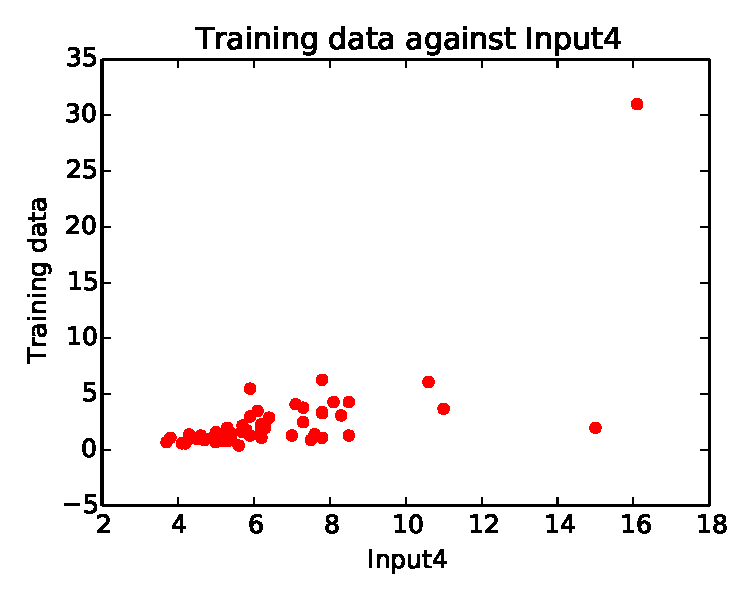
\includegraphics[width=0.25\textwidth]{../figures/auto-stat-lin-ex/lin-train-Input4.pdf}};
  \end{scope}
  \pause
  \begin{scope}[yshift=-0.25\textwidth]
    \node (raw_1) at (0, 0) {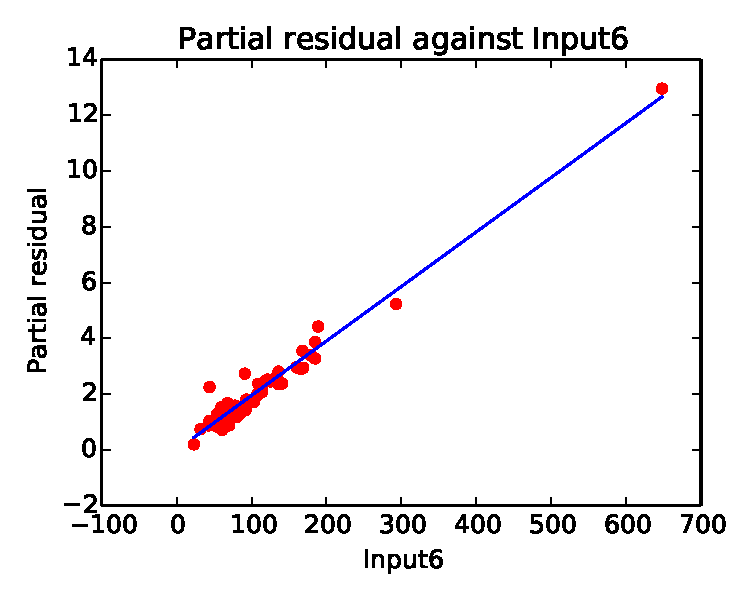
\includegraphics[width=0.25\textwidth]{../figures/auto-stat-lin-ex/lin-partial-resid-Input6.pdf}};
    \node (raw_2) [right of=raw_1] {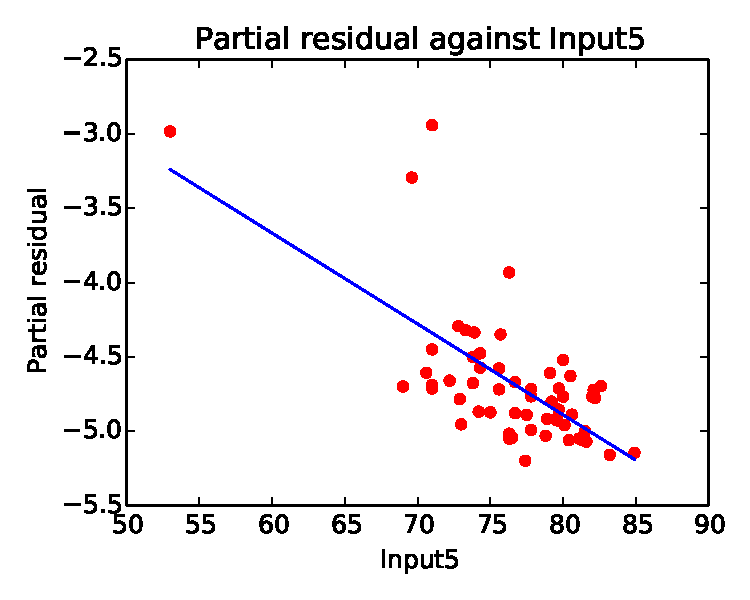
\includegraphics[width=0.25\textwidth]{../figures/auto-stat-lin-ex/lin-partial-resid-Input5.pdf}};
    \node (raw_3) [right of=raw_2] {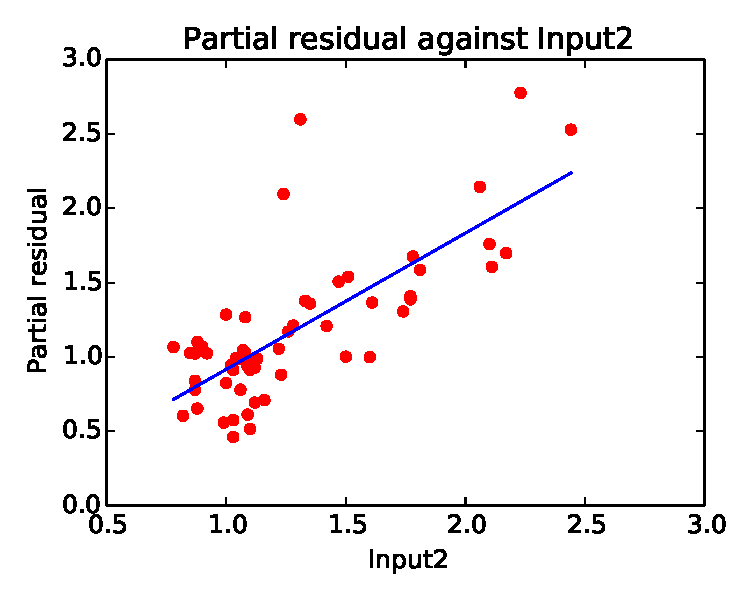
\includegraphics[width=0.25\textwidth]{../figures/auto-stat-lin-ex/lin-partial-resid-Input2.pdf}};
    \node (raw_4) [right of=raw_3] {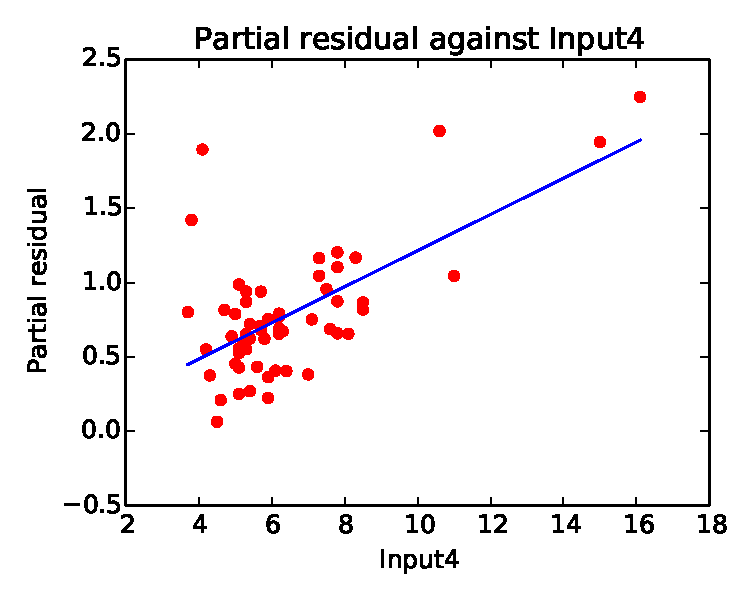
\includegraphics[width=0.25\textwidth]{../figures/auto-stat-lin-ex/lin-partial-resid-Input4.pdf}};
  \end{scope}
  \pause
  \begin{scope}[yshift=-0.45\textwidth]
    \node (quote) [text width=0.8\textwidth, align=center] at (0.4\textwidth,0)
    {``The Automatic Statistician made some sense of my data. Absolutely extraordinary.''};
  \end{scope}
\end{tikzpicture}


  \end{center}
\end{frame}

\begin{frame}{Our current focus}
    \begin{itemize}
      \item Big data
      \begin{itemize}
        \item {\bf Many data sets}
      \end{itemize}
      \item Rich models
      \begin{itemize}
        \item {\bf Automatic construction of complex functional relationships}
      \end{itemize}
      \item Interpretability
      \begin{itemize}
        \item {\bf Models are automatically described in plain English}
      \end{itemize}
      \item Good scientific philosophy
      \begin{itemize}
        \item {\bf Any model presented to a user is subjected to attempts to falsify it}
      \end{itemize}
    \end{itemize}
\end{frame}

\begin{frame}{What next?}
  \begin{center}
  \Huge
  You decide
  
  \pause
  \scriptsize (We also have some ideas of our own)
  \end{center}
\end{frame}

\begin{frame}{A system for exploratory data analysis}
    % Define block styles
  \tikzstyle{block} = [rectangle, draw, fill=blue!20, 
                       text width=4.4em, text centered, rounded corners, minimum height=3em]
  \tikzstyle{line} = [draw, -latex']
  \tikzstyle{cloud} = [draw, ellipse,fill=red!20,minimum height=2em]
    
  \begin{tikzpicture}[node distance = 2.3cm]
    \footnotesize
    % Place nodes
    \node [cloud] (data) {Data};
    \node [block, right of=data] (search) {Search};
    \node [cloud, above of=search] (language) {Language of models};
    \node [block, below of=search] (eval) {Evaluation};
    \node [cloud, right of=search] (model) {Model};
    \node [block, right of=model] (pred) {Prediction};
    \node [block, above of=pred] (trans) {Description};
    \node [block, below of=pred] (checking) {Checking};
    \node [cloud, right of=pred] (report) {Report};
    % Draw edges
    \path [line] (data) -- (search);
    \path [line] (language) -- (search);
    \path [line] (search) -- (model);
    \path [line] (search) -- (model);
    \path [line] (model.north east) -- (trans.south west);
    \path [line] (model.east) -- (pred.west);
    \path [line] (model.south east) -- (checking.north west);
    \path [line] (trans.south east) -- (report.north west);
    \path [line] (pred.east) -- (report.west);
    \path [line] (checking.north east) -- (report.south west);
    \draw[->,] (search.south east) .. controls (3.45,-1.15) .. (eval.north east);
    \draw[->,] (eval.north west) .. controls (1.15,-1.15) .. (search.south west);
  \end{tikzpicture}
\end{frame}

\begin{frame}{An entirely automatic analysis}
  \begin{center}
    \begin{tikzpicture}
      \begin{scope}[yshift=0\textwidth]
        \node (raw_data) at (-0.25\textwidth, 0) {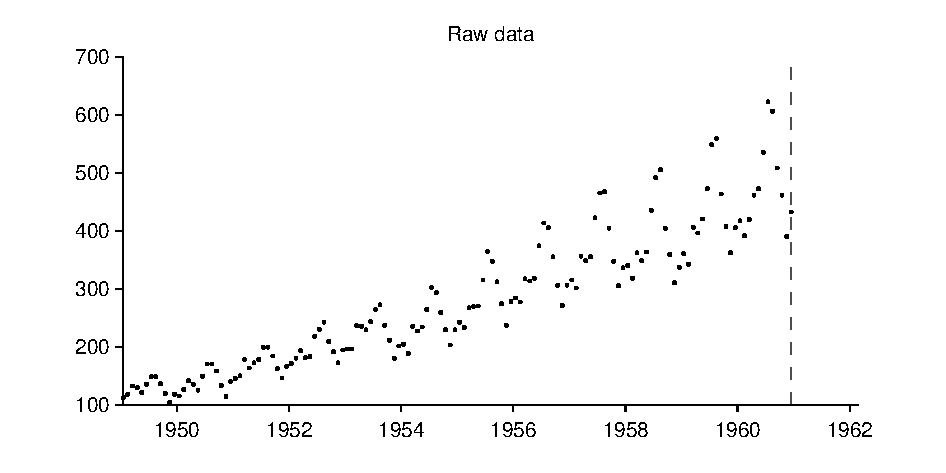
\includegraphics[width=0.45\textwidth]{../figures/01-airline/01-airline_raw_data}};
        \node (posterior) at (+0.25\textwidth, 0)  {\includegraphics[width=0.45\textwidth]{../figures/01-airline/01-airline_all}};
      \end{scope}
      \begin{scope}[yshift=-0.18\textwidth]
        \node (description) at (0, +0.03\textwidth) {\small Four additive components have been identified in the data};
        \node (component_1) at (-0.20\textwidth, -0.09\textwidth) 
              {\includegraphics[width=0.25\textwidth]{../figures/01-airline/01-airline_1}};
        \node [text width=0.4\textwidth, align=center] (component_1_text) at (-0.20\textwidth, -0.193\textwidth) 
              {\scriptsize A linearly increasing function};
        \node (component_2) at (+0.20\textwidth, -0.09\textwidth) 
              {\includegraphics[width=0.25\textwidth]{../figures/01-airline/01-airline_2}};
        \node [text width=0.4\textwidth, align=center] (component_2_text) at (+0.20\textwidth, -0.166\textwidth) 
              {\scriptsize An approximately periodic function};
        \node [text width=0.4\textwidth, align=center] (component_2_text) at (+0.20\textwidth, -0.193\textwidth) 
              {\scriptsize with a period of 1.0 years with};
        \node [text width=0.4\textwidth, align=center] (component_2_text) at (+0.20\textwidth, -0.220\textwidth) 
              {\scriptsize linearly increasing amplitude};
        \node (component_3) at (-0.20\textwidth, -0.3\textwidth) 
              {\includegraphics[width=0.25\textwidth]{../figures/01-airline/01-airline_3}};
        \node [text width=0.4\textwidth, align=center] (component_3_text) at (-0.20\textwidth, -0.393\textwidth) 
              {\scriptsize A smooth function};
        \node (component_4) at (+0.20\textwidth, -0.3\textwidth) 
              {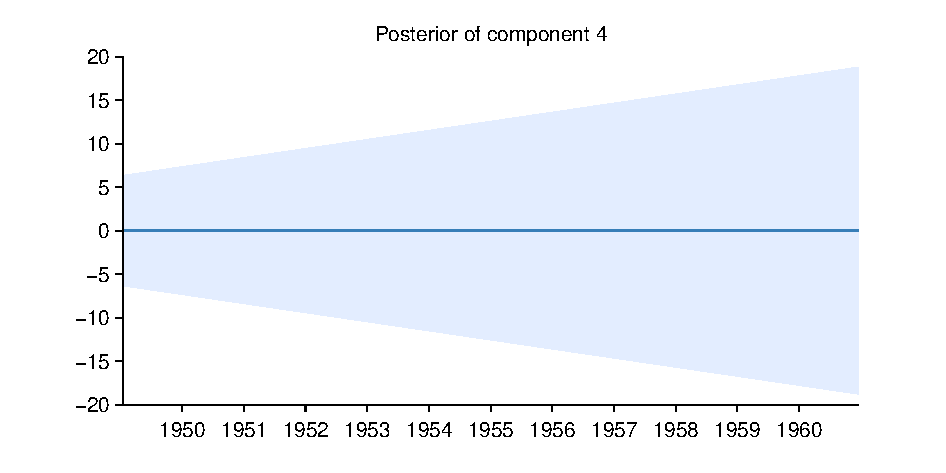
\includegraphics[width=0.25\textwidth]{../figures/01-airline/01-airline_4}};
        \node [text width=0.4\textwidth, align=center] (component_4_text) at (+0.20\textwidth, -0.3795\textwidth) 
              {\scriptsize Uncorelated noise with linearly};
        \node [text width=0.4\textwidth, align=center] (component_4_text) at (+0.20\textwidth, -0.4065\textwidth) 
              {\scriptsize increasing standard deviation};
      \end{scope}
    \end{tikzpicture}
  \end{center}
\end{frame}

\begin{frame}{Defining a language of models}
    % Define block styles
  \tikzstyle{block} = [rectangle, draw, fill=blue!20, 
                       text width=4.4em, text centered, rounded corners, minimum height=3em]
  \tikzstyle{line} = [draw, -latex']
  \tikzstyle{cloud} = [draw, ellipse,fill=red!20,minimum height=2em]
  \tikzstyle{supercloud} = [draw, ellipse,fill=red!50,minimum height=2em,]
    
  \begin{tikzpicture}[node distance = 2.3cm]
    \footnotesize
    % Place nodes
    \node [cloud] (data) {Data};
    \node [block, right of=data] (search) {Search};
    \node [supercloud, above of=search] (language) {\bf Language of models};
    \node [block, below of=search] (eval) {Evaluation};
    \node [cloud, right of=search] (model) {Model};
    \node [block, right of=model] (pred) {Prediction};
    \node [block, above of=pred] (trans) {Description};
    \node [block, below of=pred] (checking) {Checking};
    \node [cloud, right of=pred] (report) {Report};
    % Draw edges
    \path [line] (data) -- (search);
    \path [line] (language) -- (search);
    \path [line] (search) -- (model);
    \path [line] (search) -- (model);
    \path [line] (model.north east) -- (trans.south west);
    \path [line] (model.east) -- (pred.west);
    \path [line] (model.south east) -- (checking.north west);
    \path [line] (trans.south east) -- (report.north west);
    \path [line] (pred.east) -- (report.west);
    \path [line] (checking.north east) -- (report.south west);
    \draw[->,] (search.south east) .. controls (3.45,-1.15) .. (eval.north east);
    \draw[->,] (eval.north west) .. controls (1.15,-1.15) .. (search.south west);
  \end{tikzpicture}
\end{frame}

\begin{frame}{A language of Gaussian processes}
  \begin{itemize}
    \item A Gaussian process is collection of random variables, any finite number of which have a joint Gaussian distribution
    \pause
    \vspace{\baselineskip}
    \item We can write this collection of random variables as $\{f(x) : x \in \mathcal{X}\}$ \ie a function $f$ evaluated at inputs $x$
    \pause
    \vspace{\baselineskip}
    \item A \gp{} is completely specified by
    \begin{itemize}
      \item Mean function, $\mu(x)=\mathbb{E}(f(x))$
      \item Covariance / kernel function, $\kernel(x,x') = \Cov(f(x),f(x'))$
      \item Denoted $f \,\sim\, \gp{}(\mu,\kernel)$
    \end{itemize}
    \vspace{\baselineskip}
    \pause
    \item Two important facts for this talk
    \begin{itemize}
      \item Can be used to perform Bayesian (nonlinear) regression
      \item High level properties determined by kernel
    \end{itemize}
  \end{itemize}
\end{frame}

\begin{frame}{Gaussian process regression in pictures}
  \begin{itemize}
    \item Define probability distributions on functions
    \item Used to perform Bayesian (nonlinear) regression
  \end{itemize}
  \vspace{\baselineskip}
  \begin{center}
    \includegraphics<1>[width=0.8\textwidth]{../figures/lin_reg/sq_exp_prior}
    \includegraphics<2>[width=0.8\textwidth]{../figures/quad/sq_exp_1}
    \includegraphics<3>[width=0.8\textwidth]{../figures/quad/sq_exp_2}
    \includegraphics<4>[width=0.8\textwidth]{../figures/quad/sq_exp_3}
    \includegraphics<5>[width=0.8\textwidth]{../figures/quad/sq_exp_5}
    \includegraphics<6>[width=0.8\textwidth]{../figures/quad/sq_exp_10}
    \includegraphics<7>[width=0.8\textwidth]{../figures/quad/sq_exp_15}
  \end{center}
\end{frame}

\begin{frame}{Properties specified by kernel}
  \begin{itemize}
    \only<1>{\item The periodic kernel encodes for a probability distribution over periodic functions}
    \only<2>{\item The linear kernel results in a probability distribution over linear functions}
  \end{itemize}
  %\vspace{\baselineskip}
  \begin{center}
    \includegraphics<1>[width=0.8\textwidth]{../figures/quad/periodic_prior}
    \includegraphics<2>[width=0.8\textwidth]{../figures/quad/new_lin_prior}
  \end{center}
\end{frame}

\begin{frame}{The atoms of our language}  
  \newcommand{\fhbig}{1.0cm}
\newcommand{\fwbig}{1.2cm}
\newcommand{\kernpic}[1]{\includegraphics[height=\fhbig,width=\fwbig]{../figures/structure_examples/#1}}
\newcommand{\colsize}{1.7cm}
\newcommand{\sepsize}{0.0cm}

Five base kernels\dots

\vspace{\baselineskip}

\begin{tabularx}{\columnwidth}{x{\colsize}x{\colsize}x{\colsize}x{\colsize}x{\colsize}}
  \kernpic{se_kernel} & \kernpic{per_kernel} & \kernpic{lin_kernel} & \kernpic{c_kernel} & \kernpic{wn_kernel} \\
  {\footnotesize Squared \newline exp. (\kSE)} & {\footnotesize Periodic (\kPer)} & {\footnotesize Linear (\kLin)} & {\footnotesize Constant (\kC)} & {\footnotesize White \newline noise (\kWN)}
\end{tabularx}

\vspace{\baselineskip}

\dots encoding for the following types of functions

\vspace{\baselineskip}

\begin{tabularx}{\columnwidth}{x{\colsize}x{\colsize}x{\colsize}x{\colsize}x{\colsize}}
  \kernpic{se_kernel_draws} & \kernpic{per_kernel_draws_s2} & \kernpic{lin_kernel_draws} & \kernpic{c_kernel_draws} & \kernpic{wn_kernel_draws} \\
  {\footnotesize Smooth \newline functions} & {\footnotesize Periodic functions} & {\footnotesize Linear \newline functions} & {\footnotesize Constant \newline functions} & {\footnotesize Gaussian \newline noise} 
\end{tabularx}


\end{frame}

\begin{frame}{The composition rules of our language}
\begin{itemize} 
	\item Two main operations: addition, multiplication
\end{itemize}
\newcommand{\fhbig}{1.6cm}
\newcommand{\fwbig}{1.8cm}
\newcommand{\kernpic}[1]{\includegraphics[height=\fhbig,width=\fwbig]{figures/structure_examples/#1}}
\newcommand{\largeplus}{\tabbox{{\Large+}}}
\newcommand{\largeeq}{\tabbox{{\Large=}}}
\newcommand{\largetimes}{\tabbox{{\Large$\times$}}}
\begin{figure}[ht]
\centering
\renewcommand{\tabularxcolumn}[1]{>{\arraybackslash}m{#1}}
\begin{tabularx}{\columnwidth}{XXcXX}
  {\small $\kLin \times \kLin$} & \kernpic{lin_times_lin_draws} & \phantom{mm}
& {\small $\kSE \times \kPer$} & \kernpic{longse_times_per_draws_s1}
\\
   & {\small quadratic functions} & \phantom{mm}
&  & {\small locally \newline periodic}
\\ \\
%\midrule 
  {\small $\kLin + \kPer$} & \kernpic{lin_plus_per_draws} & \phantom{mm} 
& {\small $\kSE + \kPer$ } & \kernpic{se_plus_per_draws_s7}
\\
   & {\small periodic plus linear trend} & \phantom{mm}
&  & {\small periodic plus smooth trend}
\end{tabularx}
\end{figure}


\end{frame}
\begin{frame}{Modeling changepoints}
  
  Time series data often exhibit changepoints:
  
  \begin{center}
  \begin{tabular}{cc}
    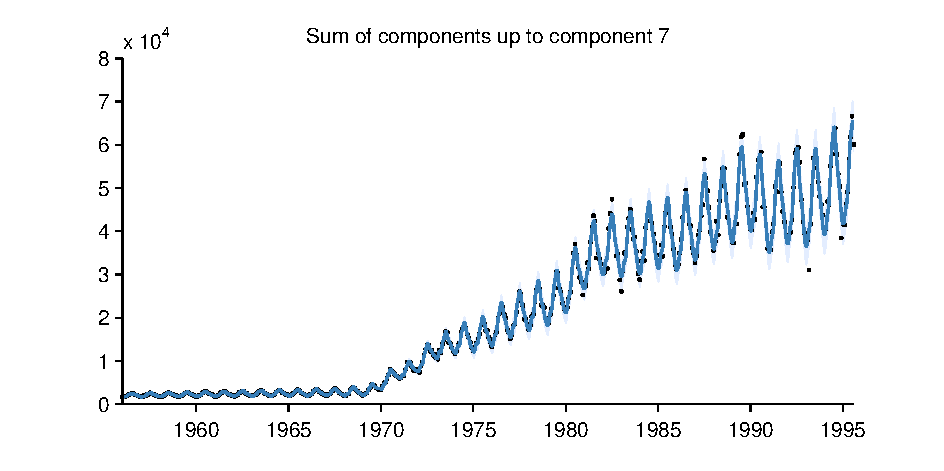
\includegraphics[width=0.4\textwidth]{../figures/09-gas-production_7_cum} &
    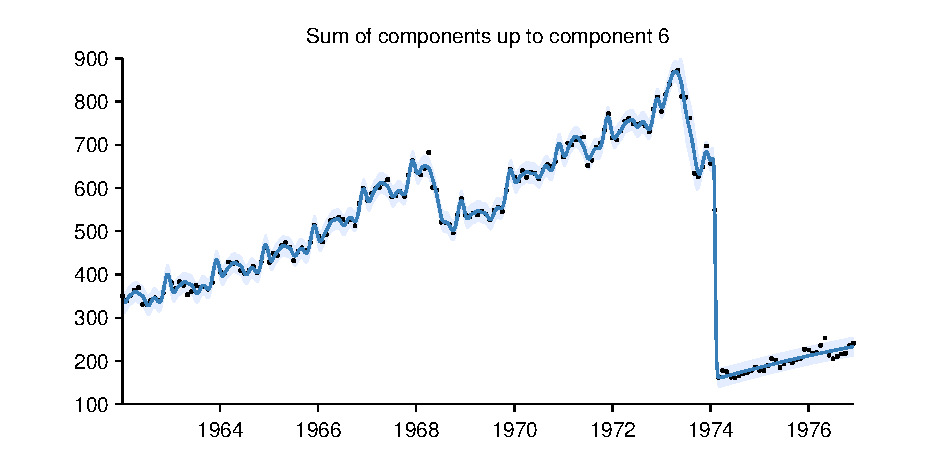
\includegraphics[width=0.4\textwidth]{../figures/07-call-centre_6_cum} 
  \end{tabular}
  \end{center}
  
  \pause

  We can model this by assuming $\textcolor{red}{f_1(x)} \sim \gp{}(0,k_1)$ and $\textcolor{blue}{f_2(x)} \sim \gp{}(0,k_2)$ and then defining
\[
f(x) = (1-\sigma(x))\, \textcolor{red}{f_1(x)} + \sigma(x)\, \textcolor{blue}{f_2(x)}
\]

where $\sigma$ is a sigmoid function between 0 and 1.
\end{frame}

\begin{frame}{Modeling changepoints}
  We can model this by assuming $\textcolor{red}{f_1(x)} \sim \gp{}(0,k_1)$ and $\textcolor{blue}{f_2(x)} \sim \gp{}(0,k_2)$ and then defining
\[
f(x) = (1-\sigma(x))\, \textcolor{red}{f_1(x)} + \sigma(x)\, \textcolor{blue}{f_2(x)}
\]

where $\sigma$ is a sigmoid function between 0 and 1.

\vspace{2\baselineskip}

Then $f \sim \gp{}(0,k)$, where
\[
k(x,x') = (1-\sigma(x)) \, \textcolor{red}{k_1(x,x')}  \, (1-\sigma(x')) + \sigma(x) \,
\textcolor{blue}{k_2(x,x')} \, \sigma(x') 
\]

We define the changepoint operator $\kernel = \kCP(\kernel_1, \kernel_2)$.

\end{frame}

\begin{frame}{An expressive language of models}
\begin{center}
\begin{tabular}{l|l}
Regression model & Kernel \\
\midrule
\gp{} smoothing & $\kSE + \kWN$ \\
Linear regression & $\kC + \kLin + \kWN$ \\
Multiple kernel learning & $\sum \kSE$ + \kWN\\
Trend, cyclical, irregular & $\sum \kSE + \sum \kPer$ + \kWN\\
Fourier decomposition & $\kC + \sum \cos$ + \kWN\\
Sparse spectrum \gp{}s & $\sum \cos$ + \kWN\\
Spectral mixture & $\sum \SE \times \cos$ + \kWN\\
Changepoints & \eg $\kCP(\kSE, \kSE) + \kWN$ \\
Heteroscedasticity & \eg $\kSE + \kLin \times \kWN$
\end{tabular}
\end{center}
Note: $\cos$ is a special case of our version of $\kPer$
\end{frame}

\begin{frame}{Language extends to multiple dimensions}
\begin{center}
\begin{tabular}{l|l}
Regression model & Kernel \\
\midrule
Multiple linear & \multirow{2}{*}{$\kC + \sum_d \kSE_d + \kWN$} \\
regression & \\
Polynomial regression & $\kC + \sum_d \prod \kSE_d + \kWN$ \\
Additive smoothing & $\sum_d \kSE_d + \kWN$ \\
ANOVA smoothing & $\sum_d \kSE_d + \sum_{d_1,d_2} \kSE_{d_1} \kSE_{d_2} + \dots$ \\
Automatic relevance & \multirow{2}{*}{$\prod_d \kSE_d +  + \kWN$} \\
determination &
\end{tabular}
\end{center}
\end{frame}

\begin{frame}{Discovering a good model via search}
    % Define block styles
  \tikzstyle{block} = [rectangle, draw, fill=blue!20, 
                       text width=4.4em, text centered, rounded corners, minimum height=3em]
  \tikzstyle{superblock} = [rectangle, draw, fill=blue!50, 
                       text width=4.4em, text centered, rounded corners, minimum height=3em]
  \tikzstyle{line} = [draw, -latex']
  \tikzstyle{cloud} = [draw, ellipse,fill=red!20,minimum height=2em]
  \tikzstyle{supercloud} = [draw, ellipse,fill=red!50,minimum height=2em]
    
  \begin{tikzpicture}[node distance = 2.3cm]
    \footnotesize
    % Place nodes
    \node [cloud] (data) {Data};
    \node [superblock, right of=data] (search) {\bf Search};
    \node [cloud, above of=search] (language) {Language};
    \node [block, below of=search] (eval) {Evaluation};
    \node [cloud, right of=search] (model) {Model};
    \node [block, right of=model] (pred) {Prediction};
    \node [block, above of=pred] (trans) {Translation};
    \node [block, below of=pred] (checking) {Checking};
    \node [cloud, right of=pred] (report) {Report};
    % Draw edges
    \path [line] (data) -- (search);
    \path [line] (language) -- (search);
    \path [line] (search) -- (model);
    \path [line] (search) -- (model);
    \path [line] (model.north east) -- (trans.south west);
    \path [line] (model.east) -- (pred.west);
    \path [line] (model.south east) -- (checking.north west);
    \path [line] (trans.south east) -- (report.north west);
    \path [line] (pred.east) -- (report.west);
    \path [line] (checking.north east) -- (report.south west);
    \draw[->,] (search.south east) .. controls (3.45,-1.15) .. (eval.north east);
    \draw[->,] (eval.north west) .. controls (1.15,-1.15) .. (search.south west);
  \end{tikzpicture}
\end{frame}

\begin{frame}{Discovering a good model via search}
  \begin{itemize}
    \item Language defined as the arbitrary composition of five base kernels ($\kWN, \kC, \kLin, \kSE, \kPer$) via three operators ($+, \times, \kCP$). 
    \vspace{\baselineskip}
    \item The space spanned by this language is open-ended and can have a high branching factor requiring a judicious search
    \vspace{\baselineskip}
    \item We propose a greedy search for its simplicity and similarity to human model-building
  \end{itemize}
\end{frame}

\begin{frame}{Example: Mauna Loa Keeling Curve}
\hspace{-1.2cm}
\only<1>{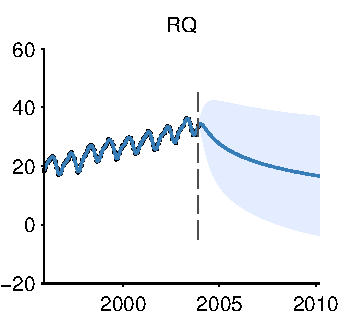
\includegraphics[width=0.4\textwidth]{../figures/11-Feb-v4-03-mauna2003-s_max_level_0/03-mauna2003-s_all_small.pdf}}
\only<2>{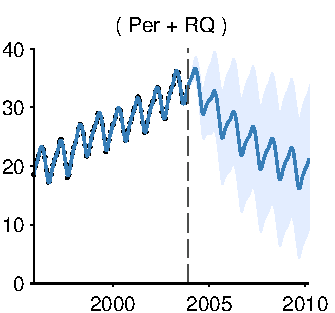
\includegraphics[width=0.4\textwidth]{../figures/11-Feb-v4-03-mauna2003-s_max_level_1/03-mauna2003-s_all_small.pdf}}
\only<3>{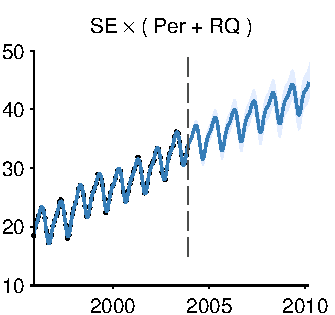
\includegraphics[width=0.4\textwidth]{../figures/11-Feb-v4-03-mauna2003-s_max_level_2/03-mauna2003-s_all_small.pdf}}
\only<4>{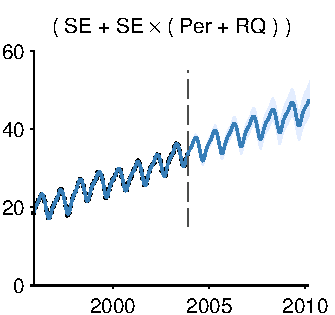
\includegraphics[width=0.4\textwidth]{../figures/11-Feb-v4-03-mauna2003-s_max_level_3/03-mauna2003-s_all_small.pdf}}

\vspace{-3.5cm}
\begin{minipage}[t][14cm][t]{1.14\linewidth}
\begin{flushleft}
\hspace{5.5cm}
\vspace{-8cm}
\makebox[\textwidth][c]{
\raisebox{10cm}{
\vspace{-8cm}
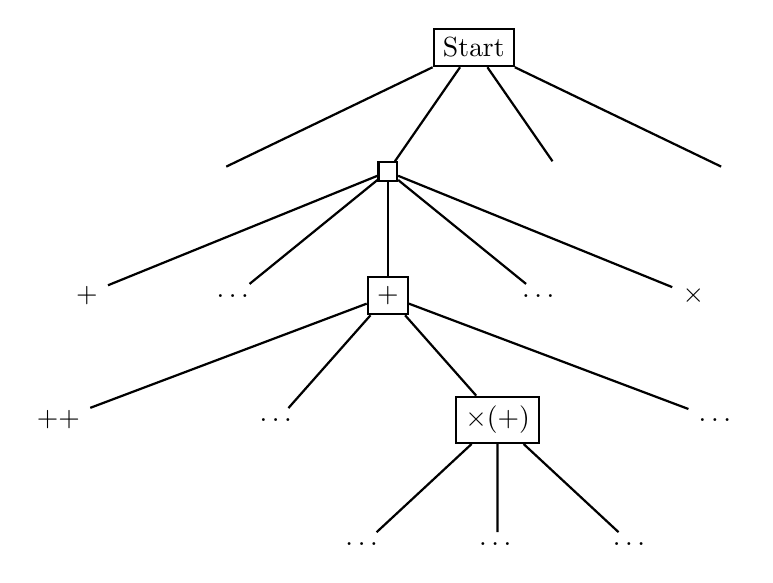
\begin{tikzpicture}
[sibling distance=0.18\columnwidth,-,thick, level distance=0.13\columnwidth]
%\footnotesize
\node[shape=rectangle,draw,thick] {Start}
%\pause
  child {node {$\SE$}}
%  fill=camlightblue!30
  child {node[shape=rectangle,draw,thick] {$\RQ$}
    [sibling distance=0.16\columnwidth]
%    {\visible<2->{ child {node {\ldots}}}}
    child [hide on=-1] {node {$\SE$ + \RQ}}
    child [hide on=-1] {node {\ldots}}
    child [hide on=-1] {node[shape=rectangle,draw,thick] {$\Per + \RQ$}
      [sibling distance=0.23\columnwidth]
      child [hide on=-2] {node {$\SE + \Per + \RQ$}}
      child [hide on=-2] {node {\ldots}}
      child [hide on=-2] {node[shape=rectangle,draw,thick] {$\SE \times (\Per + \RQ)$}
        [sibling distance=0.14\columnwidth]
        child [hide on=-3] {node {\ldots}}
        child [hide on=-3] {node {\ldots}}
        child [hide on=-3] {node {\ldots}}
      }
      child [hide on=-2] {node {\ldots}}
    }
    %child {node {$\RQ \times \SE$}}
    child [hide on=-1] {node {\ldots}}
    child [hide on=-1] {node {$\Per \times \RQ$}}
  }
  child {node {$\Lin$}}
  child {node {$\Per$}}
  ;
\end{tikzpicture}}
}\end{flushleft}
\end{minipage}
\only<4>{}
\end{frame}

\begin{frame}{Model evaluation}
    % Define block styles
  \tikzstyle{block} = [rectangle, draw, fill=blue!20, 
                       text width=4.4em, text centered, rounded corners, minimum height=3em]
  \tikzstyle{superblock} = [rectangle, draw, fill=blue!50, 
                       text width=4.4em, text centered, rounded corners, minimum height=3em]
  \tikzstyle{line} = [draw, -latex']
  \tikzstyle{cloud} = [draw, ellipse,fill=red!20,minimum height=2em]
  \tikzstyle{supercloud} = [draw, ellipse,fill=red!50,minimum height=2em]
    
  \begin{tikzpicture}[node distance = 2.3cm]
    \footnotesize
    % Place nodes
    \node [cloud] (data) {Data};
    \node [block, right of=data] (search) {Search};
    \node [cloud, above of=search] (language) {Language of models};
    \node [superblock, below of=search] (eval) {\bf Evaluation};
    \node [cloud, right of=search] (model) {Model};
    \node [block, right of=model] (pred) {Prediction};
    \node [block, above of=pred] (trans) {Description};
    \node [block, below of=pred] (checking) {Checking};
    \node [cloud, right of=pred] (report) {Report};
    % Draw edges
    \path [line] (data) -- (search);
    \path [line] (language) -- (search);
    \path [line] (search) -- (model);
    \path [line] (search) -- (model);
    \path [line] (model.north east) -- (trans.south west);
    \path [line] (model.east) -- (pred.west);
    \path [line] (model.south east) -- (checking.north west);
    \path [line] (trans.south east) -- (report.north west);
    \path [line] (pred.east) -- (report.west);
    \path [line] (checking.north east) -- (report.south west);
    \draw[->,] (search.south east) .. controls (3.45,-1.15) .. (eval.north east);
    \draw[->,] (eval.north west) .. controls (1.15,-1.15) .. (search.south west);
  \end{tikzpicture}
\end{frame}

\begin{frame}{Model evaluation}
  \begin{itemize}
    \item After proposing a new model its kernel parameters are optimised by conjugate gradients
    \vspace{\baselineskip}
    \item We evaluate each optimised model, $M$, using the \textcolor{red}{marginal likelihood} which can be computed analytically for \gp{}s
    \vspace{\baselineskip}
    \item We \textcolor{blue}{penalise} the marginal likelihood for the \textcolor{blue}{optimised kernel parameters} using the Bayesian Information Criterion (BIC):
\[
-0.5 \times \textrm{BIC}(M) = \textcolor{red}{\log p(D\,|\, M)} - \textcolor{blue}{\frac{p}{2} \log n}
\]
where $p$ is the number of kernel parameters, $D$ represents the data, and $n$ is the number of data points.
  \end{itemize}
\end{frame}

\begin{frame}{Automatic translation of models}
    % Define block styles
  \tikzstyle{block} = [rectangle, draw, fill=blue!20, 
                       text width=4.4em, text centered, rounded corners, minimum height=3em]
  \tikzstyle{superblock} = [rectangle, draw, fill=blue!50, 
                       text width=4.4em, text centered, rounded corners, minimum height=3em]
  \tikzstyle{line} = [draw, -latex']
  \tikzstyle{cloud} = [draw, ellipse,fill=red!20,minimum height=2em]
  \tikzstyle{supercloud} = [draw, ellipse,fill=red!50,minimum height=2em]
    
  \begin{tikzpicture}[node distance = 2.3cm]
    \footnotesize
    % Place nodes
    \node [cloud] (data) {Data};
    \node [block, right of=data] (search) {Search};
    \node [cloud, above of=search] (language) {Language of models};
    \node [block, below of=search] (eval) {Evaluation};
    \node [cloud, right of=search] (model) {Model};
    \node [block, right of=model] (pred) {Prediction};
    \node [superblock, above of=pred] (trans) {Translation};
    \node [block, below of=pred] (checking) {Checking};
    \node [cloud, right of=pred] (report) {Report};
    % Draw edges
    \path [line] (data) -- (search);
    \path [line] (language) -- (search);
    \path [line] (search) -- (model);
    \path [line] (search) -- (model);
    \path [line] (model.north east) -- (trans.south west);
    \path [line] (model.east) -- (pred.west);
    \path [line] (model.south east) -- (checking.north west);
    \path [line] (trans.south east) -- (report.north west);
    \path [line] (pred.east) -- (report.west);
    \path [line] (checking.north east) -- (report.south west);
    \draw[->,] (search.south east) .. controls (3.45,-1.15) .. (eval.north east);
    \draw[->,] (eval.north west) .. controls (1.15,-1.15) .. (search.south west);
  \end{tikzpicture}
\end{frame}

\begin{frame}{Automatic translation of models}
  \begin{itemize}
    \item Search can produce {\bf arbitrarily complicated models} from open-ended language but two main properties allow description to be automated
    \vspace{\baselineskip}
    \item Kernels can be {\bf decomposed} into a {\bf sum of products}
    \begin{itemize}
      \item A sum of kernels corresponds to a sum of functions
      \item Therefore, we can describe each product of kernels separately
    \end{itemize}
    \vspace{\baselineskip}
    \item Each kernel in a product modifies a model in a {\bf consistent} way
    \begin{itemize}
      \item Each kernel roughly corresponds to an adjective
    \end{itemize}
  \end{itemize}
\end{frame}

\begin{frame}{Sum of products normal form}
  %\begin{center}
  Suppose the search finds the following kernel
  \begin{align*}
    \kSE \times (\kWN \times \kLin + \kCP(\kC, \kPer))
  \end{align*}
  \pause
  The changepoint can be converted into a sum of products
  \begin{align*}
    \kSE \times (\kWN \times \kLin + \kC \times \boldsymbol{\sigma} + \kPer \times \boldsymbol{\bar\sigma})
  \end{align*}
  \pause
  Multiplication can be distributed over addition
  \begin{align*}
    \kSE \times \kWN \times \kLin + \kSE \times \kC \times \boldsymbol{\sigma} + \kSE \times \kPer \times \boldsymbol{\bar\sigma}
  \end{align*}
  \pause
  Simplification rules are applied
  \begin{align*}
    \kWN \times \kLin + \kSE \times \boldsymbol{\sigma} + \kSE \times \kPer \times \boldsymbol{\bar\sigma}
  \end{align*}
  %\end{center}
\end{frame}

\begin{frame}{Sums of kernels are sums of functions}
  If ${\textcolor{red}{f_1} \,\sim\, \gp{}(0, \textcolor{red}{\kernel_1})}$ and independently ${\textcolor{blue}{f_2} \,\sim\, \gp{}(0, \textcolor{blue}{\kernel_2})}$ then
  \begin{align*}
  \textcolor{red}{f_1} + \textcolor{blue}{f_2} \,\sim\, \gp{}(0, \textcolor{red}{\kernel_1} + \textcolor{blue}{\kernel_2})
  \end{align*}
  
\eg

\vspace{\baselineskip}

\begin{tabular}{ccccccc}
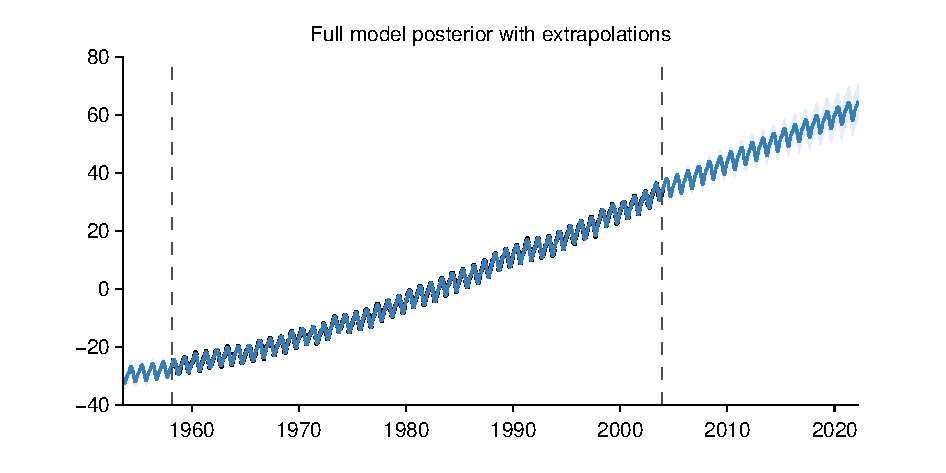
\includegraphics[trim=30 0 62 25, clip, width=0.15\textwidth]{../figures/03-mauna2003_all} &
\raisebox{0.4cm}{$=$} &
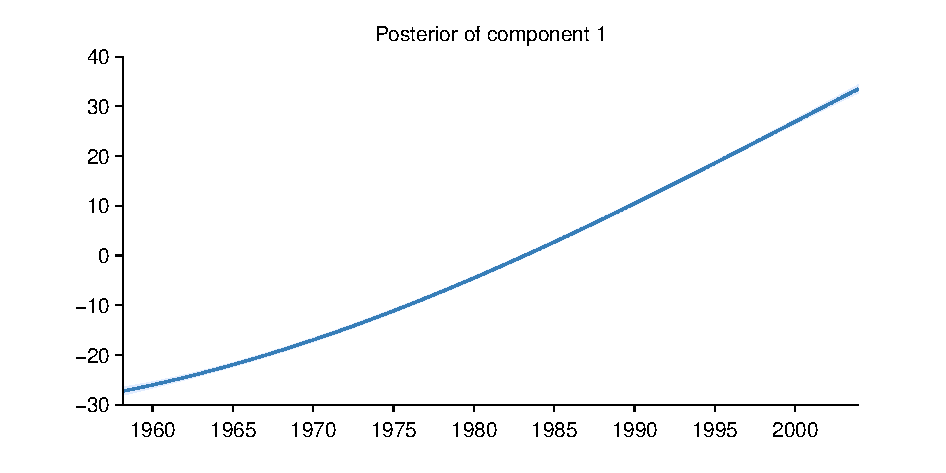
\includegraphics[trim=30 0 62 25, clip, width=0.15\textwidth]{../figures/03-mauna2003_1} &
\raisebox{0.4cm}{$+$} &
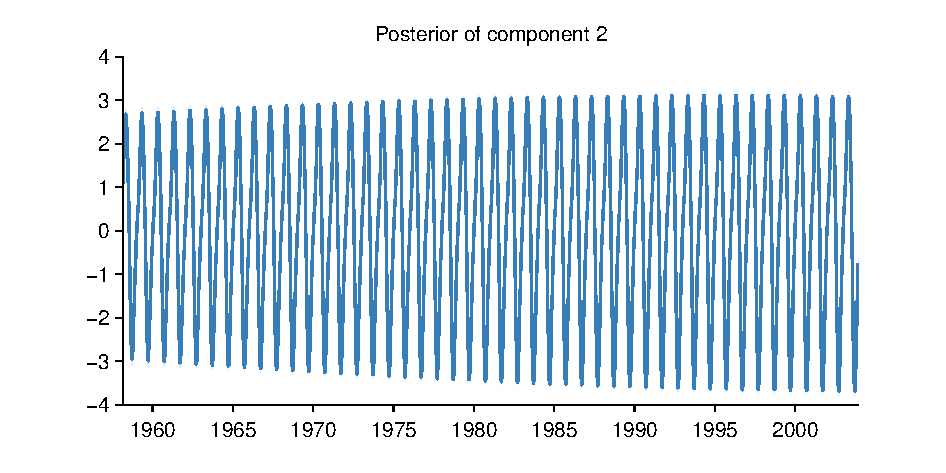
\includegraphics[trim=30 0 62 25, clip, width=0.15\textwidth]{../figures/03-mauna2003_2} &
\raisebox{0.4cm}{$+$} &
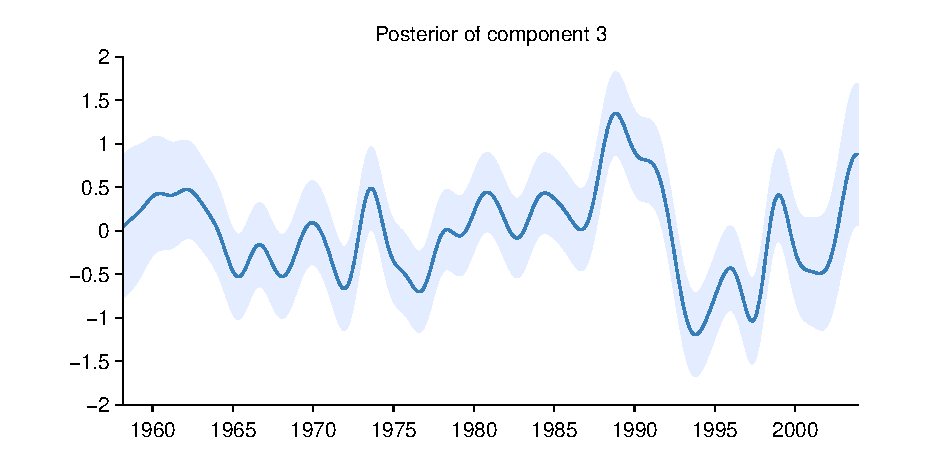
\includegraphics[trim=30 0 62 25, clip, width=0.15\textwidth]{../figures/03-mauna2003_3}
\end{tabular}

\vspace{\baselineskip}

\begin{tabular}{ccccccc}
\includegraphics[trim=30 0 62 25, clip, width=0.15\textwidth]{../figures/01-airline_all} &
\raisebox{0.4cm}{$=$} &
\includegraphics[trim=30 0 62 25, clip, width=0.15\textwidth]{../figures/01-airline_1} &
\raisebox{0.4cm}{$+$} &
\includegraphics[trim=30 0 62 25, clip, width=0.15\textwidth]{../figures/01-airline_2} &
\raisebox{0.4cm}{$+$} &
\includegraphics[trim=30 0 62 25, clip, width=0.15\textwidth]{../figures/01-airline_3}
\end{tabular}

\vspace{\baselineskip}

We can therefore describe each component separately

\end{frame}

\begin{frame}{Products of kernels}
  \begin{align*}
    \hspace*{-6mm}
    \underbrace{\kPer}_{\textnormal{\scriptsize a periodic function}} \phantom{\times 
    \underbrace{\kSE}_{\textnormal{\scriptsize whose shape changes smoothly}} \times
    \underbrace{\kLin}_{\textnormal{\scriptsize with linearly growing amplitude}} \times 
    \underbrace{\boldsymbol{\sigma}}_{\textnormal{\scriptsize until 1700}}}
  \end{align*}
  
  \vspace{\baselineskip}
  
  On their own, each kernel is described by a standard noun phrase
  
  \vspace{\baselineskip}
  
  \begin{block}{}
    \begin{tabular}{cccc}
      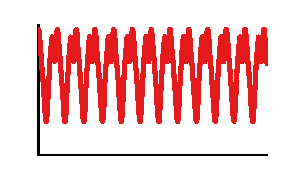
\includegraphics[width=0.2\textwidth]{../figures/trans_samples/draw_11} &
      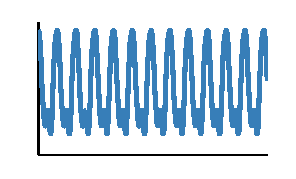
\includegraphics[width=0.2\textwidth]{../figures/trans_samples/draw_12} &
      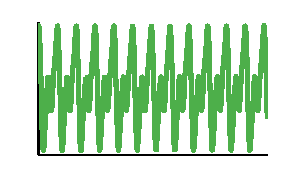
\includegraphics[width=0.2\textwidth]{../figures/trans_samples/draw_13} &
      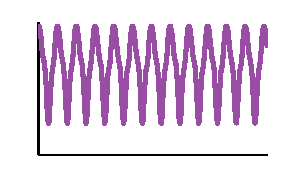
\includegraphics[width=0.2\textwidth]{../figures/trans_samples/draw_14}
    \end{tabular}
  \end{block}
\end{frame}

\begin{frame}{Products of kernels - $\kSE$}
  \begin{align*}
    \hspace*{-6mm}
    \underbrace{\kPer}_{\textnormal{\scriptsize a periodic function}} \times 
    \underbrace{\kSE}_{\textnormal{\scriptsize whose shape changes smoothly}} \phantom{\times
    \underbrace{\kLin}_{\textnormal{\scriptsize with linearly growing amplitude}} \times 
    \underbrace{\boldsymbol{\sigma}}_{\textnormal{\scriptsize until 1700}}}
  \end{align*}
  
  \vspace{\baselineskip}
  
  {\bf Multiplication by $\kSE$} removes long range correlations from a model since $\kSE(x,x')$ decreases monotonically to 0 as $|x - x'|$ increases.
  
  \vspace{\baselineskip}
  
  \begin{block}{}
    \begin{tabular}{cccc}
      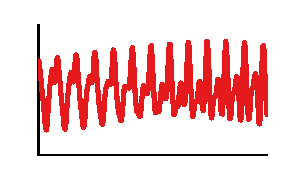
\includegraphics[width=0.2\textwidth]{../figures/trans_samples/draw_21} &
      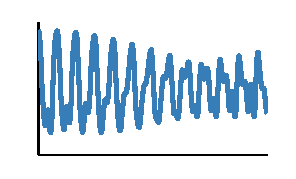
\includegraphics[width=0.2\textwidth]{../figures/trans_samples/draw_22} &
      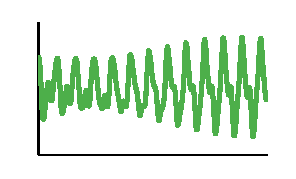
\includegraphics[width=0.2\textwidth]{../figures/trans_samples/draw_23} &
      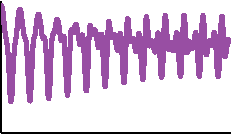
\includegraphics[width=0.2\textwidth]{../figures/trans_samples/draw_24}
    \end{tabular}
  \end{block}
\end{frame}

\begin{frame}{Products of kernels - $\kLin$}
  \begin{align*}
    \hspace*{-6mm}
    \underbrace{\kPer}_{\textnormal{\scriptsize a periodic function}} \times 
    \underbrace{\kSE}_{\textnormal{\scriptsize whose shape changes smoothly}} \times
    \underbrace{\kLin}_{\textnormal{\scriptsize with linearly growing amplitude}} \phantom{\times 
    \underbrace{\boldsymbol{\sigma}}_{\textnormal{\scriptsize until 1700}}}
  \end{align*}
  
  \vspace{\baselineskip}
  
  {\bf Multiplication by $\kLin$} is equivalent to multiplying the function being modeled by a linear function.
If $f(x) \,\sim\, \gp{}(0, \kernel)$, then $x\,f(x) \,\sim\, \gp{}\left(0, k \times \kLin \right)$.
This causes the standard deviation of the model to vary linearly without affecting the correlation.
  
  \vspace{\baselineskip}
  
  \begin{block}{}
    \begin{tabular}{cccc}
      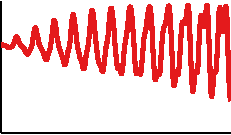
\includegraphics[width=0.2\textwidth]{../figures/trans_samples/draw_31} &
      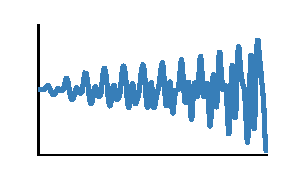
\includegraphics[width=0.2\textwidth]{../figures/trans_samples/draw_32} &
      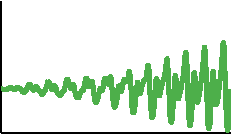
\includegraphics[width=0.2\textwidth]{../figures/trans_samples/draw_33} &
      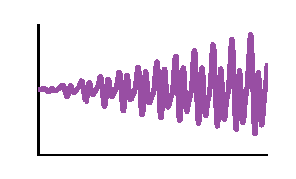
\includegraphics[width=0.2\textwidth]{../figures/trans_samples/draw_34}
    \end{tabular}
  \end{block}
\end{frame}

\begin{frame}{Products of kernels - changepoints}
  \begin{align*}
    \hspace*{-6mm}
    \underbrace{\kPer}_{\textnormal{\scriptsize a periodic function}} \times 
    \underbrace{\kSE}_{\textnormal{\scriptsize whose shape changes smoothly}} \times
    \underbrace{\kLin}_{\textnormal{\scriptsize with linearly growing amplitude}} \times 
    \underbrace{\boldsymbol{\sigma}}_{\textnormal{\scriptsize until 1700}}
  \end{align*}
  
  \vspace{\baselineskip}
  
  {\bf Multiplication by $\boldsymbol\sigma$} is equivalent to multiplying the function being modeled by a sigmoid.
  
  \vspace{\baselineskip}
  
  \begin{block}{}
    \begin{tabular}{cccc}
      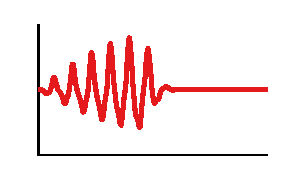
\includegraphics[width=0.2\textwidth]{../figures/trans_samples/draw_41} &
      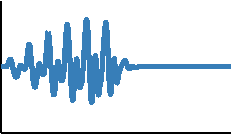
\includegraphics[width=0.2\textwidth]{../figures/trans_samples/draw_42} &
      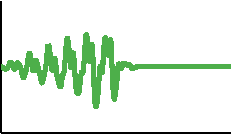
\includegraphics[width=0.2\textwidth]{../figures/trans_samples/draw_43} &
      \includegraphics[width=0.2\textwidth]{../figures/trans_samples/draw_44}
    \end{tabular}
  \end{block}
\end{frame}

\begin{frame}{Noun phrase and postmodifier forms}
  \begin{center}
    \footnotesize
    \begin{tabular}{l|l|l}
      Kernel & Noun phrase & Postmodifier phrase \\
      \midrule
      $\kWN$  & uncorrelated noise & n/a\\
      $\kC$   & constant & n/a \\
      $\kSE$  & smooth function & whose shape changes smoothly\\
      $\kPer$ & periodic function & modulated by a periodic function\\
      $\kLin$ & linear function & with linearly varying amplitude\\ 
      $\prod_k \kLin^{(k)}$ & polynomial & with polynomially varying amplitude\\
      $\prod_k \boldsymbol{\sigma}^{(k)}$ & n/a & which applies until / from [changepoint]
    \end{tabular}
  \end{center}
\end{frame}

\begin{frame}{Why are pictures not enough?}
  \begin{center}
    \begin{tikzpicture}[]
  \begin{scope}[yshift=+0.35\textwidth]
    \node (quote) [text width=0.7\textwidth, align=center] at (0.25\textwidth,0)
    {``If you can't explain it simply, you don't understand it well enough''};
  \end{scope}
  \pause
  \begin{scope}[yshift=0\textwidth]
    \begin{scope}[xshift=0.0\textwidth]
      \node [mybox] (box){
        \fbox{\includegraphics[trim=0cm 0cm 0cm 0cm, clip, width=0.35\textwidth]{../figures/old-gpss/03-mauna2003-s_3.pdf}}
      };
    \end{scope}
    \pause  
    \begin{scope}[xshift=0.25\textwidth]
    \draw[->,thick] (-0.04\textwidth,0.05\textwidth) -- (0.04\textwidth,0.11\textwidth); 
    \draw[->,thick] (-0.04\textwidth,-0.05\textwidth) -- (0.04\textwidth,-0.11\textwidth); 
    \end{scope}
    \begin{scope}[xshift=0.5\textwidth]
      \begin{scope}[yshift=+0.15\textwidth]
      \node [mybox] (box){
        \fbox{\includegraphics[trim=0cm 0cm 0cm 0cm, clip, width=0.35\textwidth]{../figures/03-mauna2003_3}}
      };
      \end{scope}
      \node[font=\LARGE] at (0,0) {$+$};
      \begin{scope}[yshift=-0.15\textwidth]
      \node [mybox] (box){
        \fbox{\includegraphics[trim=0cm 0cm 0cm 0cm, clip, width=0.35\textwidth]{../figures/03-mauna2003_4}}
      };
      \end{scope}
    \end{scope}
  \end{scope}
\end{tikzpicture}


  \end{center}
\end{frame}

\begin{frame}{Automatically generated reports}
    % Define block styles
  \tikzstyle{block} = [rectangle, draw, fill=blue!20, 
                       text width=4.4em, text centered, rounded corners, minimum height=3em]
  \tikzstyle{superblock} = [rectangle, draw, fill=blue!50, 
                       text width=4.4em, text centered, rounded corners, minimum height=3em]
  \tikzstyle{line} = [draw, -latex']
  \tikzstyle{cloud} = [draw, ellipse,fill=red!20,minimum height=2em]
  \tikzstyle{supercloud} = [draw, ellipse,fill=red!50,minimum height=2em]
    
  \begin{tikzpicture}[node distance = 2.3cm]
    \footnotesize
    % Place nodes
    \node [cloud] (data) {Data};
    \node [block, right of=data] (search) {Search};
    \node [cloud, above of=search] (language) {Language of models};
    \node [block, below of=search] (eval) {Evaluation};
    \node [cloud, right of=search] (model) {Model};
    \node [block, right of=model] (pred) {Prediction};
    \node [block, above of=pred] (trans) {Description};
    \node [block, below of=pred] (checking) {Checking};
    \node [supercloud, right of=pred] (report) {\bf Report};
    % Draw edges
    \path [line] (data) -- (search);
    \path [line] (language) -- (search);
    \path [line] (search) -- (model);
    \path [line] (search) -- (model);
    \path [line] (model.north east) -- (trans.south west);
    \path [line] (model.east) -- (pred.west);
    \path [line] (model.south east) -- (checking.north west);
    \path [line] (trans.south east) -- (report.north west);
    \path [line] (pred.east) -- (report.west);
    \path [line] (checking.north east) -- (report.south west);
    \draw[->,] (search.south east) .. controls (3.45,-1.15) .. (eval.north east);
    \draw[->,] (eval.north west) .. controls (1.15,-1.15) .. (search.south west);
  \end{tikzpicture}
\end{frame}

\begin{frame}{Example: Solar irradiance}
\newcommand{\wmgd}{0.5\columnwidth}
\newcommand{\hmgd}{3.0cm}
\newcommand{\mdrd}{../figures/02-solar}
\newcommand{\mbm}{\hspace{-0.3cm}}
{\footnotesize
This component is constant.
}

\vspace{\baselineskip}

\begin{tabular}{cc}
\mbm \includegraphics[width=\wmgd,height=\hmgd]{\mdrd/02-solar_1} & \includegraphics[width=\wmgd,height=\hmgd]{\mdrd/02-solar_1_cum}
\end{tabular}
\end{frame}

\begin{frame}{Example: Solar irradiance}
\newcommand{\wmgd}{0.5\columnwidth}
\newcommand{\hmgd}{3.0cm}
\newcommand{\mdrd}{../figures/02-solar}
\newcommand{\mbm}{\hspace{-0.3cm}}
{\footnotesize
This component is constant.
This component applies from 1644 until 1713.
}

\vspace{\baselineskip}

\begin{tabular}{cc}
\mbm \includegraphics[width=\wmgd,height=\hmgd]{\mdrd/02-solar_2} & \includegraphics[width=\wmgd,height=\hmgd]{\mdrd/02-solar_2_cum}
\end{tabular}
\end{frame}

\begin{frame}{Example: Solar irradiance}
\newcommand{\wmgd}{0.5\columnwidth}
\newcommand{\hmgd}{3.0cm}
\newcommand{\mdrd}{../figures/02-solar}
\newcommand{\mbm}{\hspace{-0.3cm}}
{\footnotesize
This component is a smooth function with a typical lengthscale of 23.1 years.
This component applies until 1643 and from 1716 onwards.
}

\vspace{\baselineskip}

\begin{tabular}{cc}
\mbm \includegraphics[width=\wmgd,height=\hmgd]{\mdrd/02-solar_3} & \includegraphics[width=\wmgd,height=\hmgd]{\mdrd/02-solar_3_cum}
\end{tabular}
\end{frame}

\begin{frame}{Example: Solar irradiance}
\newcommand{\wmgd}{0.5\columnwidth}
\newcommand{\hmgd}{3.0cm}
\newcommand{\mdrd}{../figures/02-solar}
\newcommand{\mbm}{\hspace{-0.3cm}}
{\footnotesize
This component is approximately periodic with a period of 10.8 years.
Across periods the shape of this function varies smoothly with a typical lengthscale of 36.9 years.
The shape of this function within each period is very smooth and resembles a sinusoid.
This component applies until 1643 and from 1716 onwards.
}

\vspace{\baselineskip}

\begin{tabular}{cc}
\mbm \includegraphics[width=\wmgd,height=\hmgd]{\mdrd/02-solar_4} & \includegraphics[width=\wmgd,height=\hmgd]{\mdrd/02-solar_4_cum}
\end{tabular}
\end{frame}

\begin{frame}{Predictive performance}
    % Define block styles
  \tikzstyle{block} = [rectangle, draw, fill=blue!20, 
                       text width=4.4em, text centered, rounded corners, minimum height=3em]
  \tikzstyle{superblock} = [rectangle, draw, fill=blue!50, 
                       text width=4.4em, text centered, rounded corners, minimum height=3em]
  \tikzstyle{line} = [draw, -latex']
  \tikzstyle{cloud} = [draw, ellipse,fill=red!20,minimum height=2em]
  \tikzstyle{supercloud} = [draw, ellipse,fill=red!50,minimum height=2em]
    
  \begin{tikzpicture}[node distance = 2.3cm]
    \footnotesize
    % Place nodes
    \node [cloud] (data) {Data};
    \node [block, right of=data] (search) {Search};
    \node [cloud, above of=search] (language) {Language of models};
    \node [block, below of=search] (eval) {Evaluation};
    \node [cloud, right of=search] (model) {Model};
    \node [superblock, right of=model] (pred) {Prediction};
    \node [block, above of=pred] (trans) {Description};
    \node [block, below of=pred] (checking) {Checking};
    \node [cloud, right of=pred] (report) {Report};
    % Draw edges
    \path [line] (data) -- (search);
    \path [line] (language) -- (search);
    \path [line] (search) -- (model);
    \path [line] (search) -- (model);
    \path [line] (model.north east) -- (trans.south west);
    \path [line] (model.east) -- (pred.west);
    \path [line] (model.south east) -- (checking.north west);
    \path [line] (trans.south east) -- (report.north west);
    \path [line] (pred.east) -- (report.west);
    \path [line] (checking.north east) -- (report.south west);
    \draw[->,] (search.south east) .. controls (3.45,-1.15) .. (eval.north east);
    \draw[->,] (eval.north west) .. controls (1.15,-1.15) .. (search.south west);
  \end{tikzpicture}
\end{frame}

\begin{frame}{Good predictive performance as well}
  \begin{block}{Standardised RMSE over 13 data sets}
  \includegraphics[width=0.99\textwidth]{../figures/box_extrap_wide}\\
  \begin{itemize}
    \item Tweaks can be made to the algorithm to improve accuracy or interpretability of models produced\ldots
    \vspace{\baselineskip}
    \item \ldots but both methods are highly competitive at extrapolation (shown above) and interpolation
  \end{itemize}
  \end{block}
\end{frame}

\begin{frame}{Model checking / criticism}
    % Define block styles
  \tikzstyle{block} = [rectangle, draw, fill=blue!20, 
                       text width=4.4em, text centered, rounded corners, minimum height=3em]
  \tikzstyle{superblock} = [rectangle, draw, fill=blue!50, 
                       text width=4.4em, text centered, rounded corners, minimum height=3em]
  \tikzstyle{line} = [draw, -latex']
  \tikzstyle{cloud} = [draw, ellipse,fill=red!20,minimum height=2em]
  \tikzstyle{supercloud} = [draw, ellipse,fill=red!50,minimum height=2em]
    
  \begin{tikzpicture}[node distance = 2.3cm]
    \footnotesize
    % Place nodes
    \node [cloud] (data) {Data};
    \node [block, right of=data] (search) {Search};
    \node [cloud, above of=search] (language) {Language of models};
    \node [block, below of=search] (eval) {Evaluation};
    \node [cloud, right of=search] (model) {Model};
    \node [block, right of=model] (pred) {Prediction};
    \node [block, above of=pred] (trans) {Description};
    \node [superblock, below of=pred] (checking) {Checking};
    \node [cloud, right of=pred] (report) {Report};
    % Draw edges
    \path [line] (data) -- (search);
    \path [line] (language) -- (search);
    \path [line] (search) -- (model);
    \path [line] (search) -- (model);
    \path [line] (model.north east) -- (trans.south west);
    \path [line] (model.east) -- (pred.west);
    \path [line] (model.south east) -- (checking.north west);
    \path [line] (trans.south east) -- (report.north west);
    \path [line] (pred.east) -- (report.west);
    \path [line] (checking.north east) -- (report.south west);
    \draw[->,] (search.south east) .. controls (3.45,-1.15) .. (eval.north east);
    \draw[->,] (eval.north west) .. controls (1.15,-1.15) .. (search.south west);
  \end{tikzpicture}
\end{frame}

\begin{frame}{Is this model `correct'?}
\newcommand{\wmgd}{0.5\columnwidth}
\newcommand{\hmgd}{3.0cm}
\newcommand{\mdrd}{../figures/11-unemployment}
\newcommand{\mbm}{\hspace{-0.3cm}}
\begin{tabular}{cc}
\mbm \includegraphics[width=\wmgd,height=\hmgd]{\mdrd/11-unemployment_raw_data} & \includegraphics[width=\wmgd,height=\hmgd]{\mdrd/11-unemployment_all}
\end{tabular}

{\footnotesize
\begin{itemize}

  \item A very smooth monotonically increasing function. 

  \item An approximately periodic function with a period of 1.0 years. 

  \item A smooth function. 

  \item A smooth function. 

  \item Uncorrelated noise. 

\end{itemize}
}
\end{frame}

\begin{frame}{Model criticism}
  \begin{itemize}
    \item Model criticism attempts to answer the question `Is this model wrong?'
    \begin{itemize}
      \item Formalised as, `could the data have been generated by this model?'
    \end{itemize}
    \vspace{\baselineskip}
    \item Typically answered by choosing a statistic by which to measure whether data is extreme
    \begin{itemize}
      \item Can then compute $p$-values to quantify surprise
      \item $p(\textrm{Data}) = \mathbb{P}(T(\textrm{Hypothetical data}) > T(\textrm{Data}) \,|\, \textrm{Model})$
    \end{itemize}
    \vspace{\baselineskip}
    \item How would an automatic system choose this statistic?
  \end{itemize}
\end{frame}

\begin{frame}{Potential solution: Try many statistics}

\begin{itemize}
  \item $p$-values of several statistics for each model component
  \item Mea culpa these $p$-values are unadjusted for multiple comparisons, but they are also uncalibrated (they are conservative)
\end{itemize}

\vspace{\baselineskip}

\begin{center}
\begin{tabular}{|r|rr|rr|rr|}
\hline
 & \multicolumn{2}{c|}{ACF} & \multicolumn{2}{c|}{Periodogram} & \multicolumn{2}{c|}{QQ} \\
\bf{\#} & {min} & {min loc} & {max} & {max loc} & {max} & {min}\\
\hline

1 & \textcolor{gray}{0.502} & \textcolor{gray}{0.582} & \textcolor{gray}{0.341} & \textcolor{gray}{0.413} & \textcolor{gray}{0.341} & \textcolor{gray}{0.679}\\

2 & \textcolor{gray}{0.802} & \textcolor{gray}{0.199} & \textcolor{gray}{0.558} & \textcolor{gray}{0.630} & 0.049 & \textcolor{gray}{0.785}\\

3 & \textcolor{gray}{0.251} & \textcolor{gray}{0.475} & \textcolor{gray}{0.799} & \textcolor{gray}{0.447} & \textcolor{gray}{0.534} & \textcolor{gray}{0.769}\\

4 & \textcolor{gray}{0.527} & \textcolor{gray}{0.503} & \textcolor{gray}{0.504} & \textcolor{gray}{0.481} & \textcolor{gray}{0.430} & \textcolor{gray}{0.616}\\

5 & \textcolor{gray}{0.493} & \textcolor{gray}{0.477} & \textcolor{gray}{0.503} & \textcolor{gray}{0.487} & \textcolor{gray}{0.518} & \textcolor{gray}{0.381}\\

\hline
\end{tabular}
\end{center}

\end{frame}

\begin{frame}{Example: Identifying outliers}
  \newcommand{\wmgd}{0.5\columnwidth}
  \newcommand{\hmgd}{3.0cm}
  \newcommand{\mdrd}{../figures/11-unemployment} 
  \newcommand{\mbm}{\hspace{-0.3cm}}
The following discrepancies between the prior and posterior distributions for this component have been detected.
\begin{itemize}
    \item The qq plot has an unexpectedly large positive deviation from equality ($x = y$). This discrepancy has an estimated $p$-value of 0.049.
\end{itemize}

\vspace{\baselineskip}

\begin{tabular}{cc}
\mbm \includegraphics[width=\wmgd,height=\hmgd]{\mdrd/11-unemployment_2} & 
\mbm \includegraphics[width=\wmgd,height=\hmgd]{\mdrd/11-unemployment_qq_bands_2}
\end{tabular}
\end{frame}

\begin{frame}{What next?}
 \begin{itemize}
   \item Plenty of ways to extend this line of work \eg
   \begin{itemize}
     \item Reducing the computational cost of model search
     \item Increasing the expressivity of the modelling language (\eg monotonicity, positive functions)
     \item Extending descriptions to multi-dimensional functions
     \item Different likelihoods (\eg outlier models)
     \item Different types of data (\eg collections of exchangeable arrays)
     \item Missing data
     \item Building causal models of multivariate data with complex functional relationships
     \item \dots
   \end{itemize}
   \vspace{\baselineskip}
   \item How can we tie all of this together?
 \end{itemize}
\end{frame}

\begin{frame}{An API for statistical modelling}
  \begin{itemize}
    \item APIs for prediction implemented by \eg  Google prediction API, auto-WEKA, \dots
    \begin{itemize}
      \item Essentially implement the functions train and predict
      \item Highly modular
    \end{itemize}
    \vspace{\baselineskip}
    \item We have started implementing some additional functions
    \begin{itemize}
      \item describe
      \item criticise / check
    \end{itemize}
    \vspace{\baselineskip}
    \item What else is needed and how can we keep it modular?
  \end{itemize}
\end{frame}

\begin{frame}{What next?}
  \begin{center}
  \large
  Where could an extension of this system be applied?
  \end{center}
\end{frame}

\begin{frame}{Thanks}
  \begin{center}
  \Huge
  Thanks
  \end{center}
\end{frame}

\begin{frame}{Appendix}
\end{frame}

\begin{frame}{Zero mean Gaussian processes}
  \begin{itemize}
    \item It is common practice to use a zero mean function since the mean can be marginalised out
  \begin{itemize}
    \item Suppose, ${f(x) \,|\, a \,\sim\, \gp{}(a \times \mu(x), \kernel(x,x'))}$ where $a \,\sim\, \mathcal{N}(0,1)$
    \item Then equivalently, $f(x) \,\sim\, \gp{}(0, \mu(x)\mu(x') + \kernel(x,x'))$
  \end{itemize}
  \vspace{\baselineskip}
  \pause
  \item We therefore define a language of \gp{} regression models by
specifying a {\bf language of kernels}
  \vspace{\baselineskip}
  \pause
  \item The choice of kernel has a large impact on the inductive bias
  \end{itemize}
\end{frame}

\begin{frame}{Kernel strongly affects extrapolation}
  \begin{center}
    \only<1>{Long lengthscale SE \\ Slowly varying and smooth}
    \only<2>{Short lengthscale SE \\ Quickly varying and smooth}
    \only<3>{Long lengthscale SE + Short lengthscale SE \\ Sum of slowly and quickly varying smooth functions}
    \only<4>{SE + SE + SE + SE $\times$ Periodic \\ Sum of smooth and approximately periodic functions}
  \end{center}
  \begin{center}
    \includegraphics<1>[width=0.8\textwidth]{../figures/mauna-plots/SE-long.pdf}
    \includegraphics<2>[width=0.8\textwidth]{../figures/mauna-plots/SE-short.pdf}
    \includegraphics<3>[width=0.8\textwidth]{../figures/mauna-plots/SE-SE.pdf}
    \includegraphics<4>[width=0.8\textwidth]{../figures/mauna-plots/Complex.pdf}
  \end{center}
\end{frame}

\begin{frame}{Example: Airline passenger volume}
\newcommand{\wmgd}{0.5\columnwidth}
\newcommand{\hmgd}{3.0cm}
\newcommand{\mdrd}{../figures/01-airline}
\newcommand{\mbm}{\hspace{-0.3cm}}
\begin{tabular}{cc}
\mbm \includegraphics[width=\wmgd,height=\hmgd]{\mdrd/01-airline_raw_data} & \includegraphics[width=\wmgd,height=\hmgd]{\mdrd/01-airline_all}
\end{tabular}

{\footnotesize
Four additive components have been identified in the data
\begin{itemize}

  \item A linearly increasing function. 

  \item An approximately periodic function with a period of 1.0 years and with linearly increasing amplitude. 

  \item A smooth function. 

  \item Uncorrelated noise with linearly increasing standard deviation. 

\end{itemize}
}
\end{frame}

\begin{frame}{Example: Airline passenger volume}
\newcommand{\wmgd}{0.5\columnwidth}
\newcommand{\hmgd}{3.0cm}
\newcommand{\mdrd}{../figures/01-airline}
\newcommand{\mbm}{\hspace{-0.3cm}}
{\footnotesize
This function is very smooth and monotonically increasing.
}

\vspace{\baselineskip}

\begin{tabular}{cc}
\mbm \includegraphics[width=\wmgd,height=\hmgd]{\mdrd/01-airline_1} & \includegraphics[width=\wmgd,height=\hmgd]{\mdrd/01-airline_1_cum}
\end{tabular}
\end{frame}

\begin{frame}{Example: Airline passenger volume}
\newcommand{\wmgd}{0.5\columnwidth}
\newcommand{\hmgd}{3.0cm}
\newcommand{\mdrd}{../figures/01-airline}
\newcommand{\mbm}{\hspace{-0.3cm}}
{\footnotesize
This component is approximately periodic with a period of 1.0 years and varying amplitude.
Across periods the shape of this function varies very smoothly.
The amplitude of the function increases approximately linearly.
The shape of this function within each period has a typical lengthscale of 6.1 weeks.
}

\vspace{\baselineskip}

\begin{tabular}{cc}
\mbm \includegraphics[width=\wmgd,height=\hmgd]{\mdrd/01-airline_2} & \includegraphics[width=\wmgd,height=\hmgd]{\mdrd/01-airline_2_cum}
\end{tabular}
\end{frame}

\begin{frame}{Example: Airline passenger volume}
\newcommand{\wmgd}{0.5\columnwidth}
\newcommand{\hmgd}{3.0cm}
\newcommand{\mdrd}{../figures/01-airline}
\newcommand{\mbm}{\hspace{-0.3cm}}
{\footnotesize
This component is a smooth function with a typical lengthscale of 8.1 months.
}

\vspace{\baselineskip}

\begin{tabular}{cc}
\mbm \includegraphics[width=\wmgd,height=\hmgd]{\mdrd/01-airline_3} & \includegraphics[width=\wmgd,height=\hmgd]{\mdrd/01-airline_3_cum}
\end{tabular}
\end{frame}

\begin{frame}{Example: Airline passenger volume}
\newcommand{\wmgd}{0.5\columnwidth}
\newcommand{\hmgd}{3.0cm}
\newcommand{\mdrd}{../figures/01-airline}
\newcommand{\mbm}{\hspace{-0.3cm}}
{\footnotesize
This component models uncorrelated noise.
The standard deviation of the noise increases linearly.
}

\vspace{\baselineskip}

\begin{tabular}{cc}
\mbm \includegraphics[width=\wmgd,height=\hmgd]{\mdrd/01-airline_4} & \includegraphics[width=\wmgd,height=\hmgd]{\mdrd/01-airline_4_cum}
\end{tabular}
\end{frame}
  
\end{document}

\begin{frame}{Title}
  \begin{itemize}
    \item Content
    \vspace{\baselineskip}
    \item Content
    \vspace{\baselineskip}
    \item Content
    \begin{itemize}
       \item Content
       \item Content
     \end{itemize}
  \end{itemize}
\end{frame}

\begin{frame}{Agenda}
  \begin{itemize}
    \item Quick introduction to Gaussian processes for regression
    \vspace{\baselineskip}
    \item A compositional language of regression models
    \vspace{\baselineskip}
    \item Searching through this space
    \vspace{\baselineskip}
    \item Automatically describing any model in natural language
    \vspace{\baselineskip}
    \item Examples of automatically generated output and model checking
    \vspace{\baselineskip}
    \item Future directions and challenges
  \end{itemize}
\end{frame}